\documentclass[11pt,letterpaper,notitlepage]{classnotes}
\pagestyle{plain}
\usepackage{classnotes}
\usepackage{latexsym,exscale,amsfonts,amsmath,amssymb,array}
\usepackage{gensymb}
\usepackage{mathtools}
\usepackage{multirow}
\usepackage{mdframed}
\usepackage{listings}
\usepackage{comment,ulem}
\newcommand{\red}[1]{{\textcolor{red}{#1}}}
\newcommand{\blue}[1]{{\textcolor{blue}{#1}}}
\newcommand\tab[1][1cm]{\hspace*{#1}}


\setlength{\topmargin}{-2.3cm}
\setlength{\textheight}{24.8cm}
\setlength{\oddsidemargin}{-0.5cm}
\setlength{\textwidth}{17cm}
\setlength{\parindent}{0cm}
% set up 1 inch margins
\usepackage[margin=1in]{geometry}

\setlength{\parskip}{.15cm}
\newcommand{\totaldiffx}{\frac{d}{dx}}
\newcommand{\pardiffx}{\frac{\partial}{\partial x}}
\newcommand{\luft}{\:\!}

\newcommand{\ze}{\mbox{Z$_e$}}
\newcommand{\emacs}{\mbox{\sc emacs}}

\usepackage{pgf}
\usepackage{tikz}
\usepackage{framed}
\usepackage{array}
\usepackage{graphicx}
\usepackage{xcolor}
\usepackage[latin1]{inputenc}
\usepackage{mathpazo}
\usepackage[T1]{fontenc}
\usepackage{chapterbib}
\usepackage[comma,numbers,sort&compress,sectionbib]{natbib}
\usepackage[colorlinks,linkcolor=blue,citecolor=blue]{hyperref}



\newcommand{\todo}[1]{{\color{red}$\blacksquare$~\textsf{[TODO: #1]}}}  

\author{The Super Duper Awesome Graduate Students of Astronomy, Physics \& Geology}
\shortauthor{Narayanan}
\title{AST 6245 -- Radiative Processes in  Astrophysics}
\email{desika.narayanan@ufl.edu}

\bibliographystyle{plainnat}

\begin{document}

\maketitle
\thispagestyle{empty}

\begin{center}
\noindent {\bf Review of Lecture Notes for Spring Term 2020}
\end{center}
\vskip1cm

\noindent 


\newpage

\tableofcontents

\pagebreak
\chapter{Spontaneous Emission, Stimulated Emission, and Absorption}
\section{Einstein Coefficients}

Einstein coefficients express the probability of emission/absorption of light by an atom/molecule. The A coefficients tells us about the rate of spontaneous emission of light, and the Bs about absorption and stimulated emission of light. Anytime we are talking about emission, we use the index $ul$, which means that the electron moved from a more energetic state to a lower one, allowing then the emission of a photon. When referring to an absorption, we use the index $lu$, which means the opposite: electron getting more energetic and moving up to a higher state due to the absorption of a photon. Following this, we have the following Einstein coefficients:
\\
\\$B_{lu}$ = Einstein absorption [$s^{-1}\;erg^{-1}\;cm^2\;str$]
\\$B_{ul} =$ Einstein stimulated emission [$s^{-1}\;erg^{-1}\;cm^2\;str$]
\\$A_{ul} =$ Einstein spontaneous emission [$s^{-1}$]
\\
\\We can relate those coefficients as expressed below:
\\
\\$g_lB_{lu} = g_u B_{ul}$
\\
\\$B_{ul} = \frac{c^3}{8\pi h \nu^3}$
\\
\\$B_{lu} = \frac{g_u}{g_l} \frac{c^3}{8\pi h \nu^3} A_{ul}$


The intensity for a determined frequency $\nu$ is
\\$B_{\nu} = \frac{\frac{A_{ul}}{B_{ul}}}{\frac{g_l B_{lu}}{g_u B_{ul}} \exp{(\frac{h\nu}{KT})}-1}$

Also:
\\$\frac{n_l}{n_u} = \frac{g_l}{g_u}e^{h\nu/kT}$


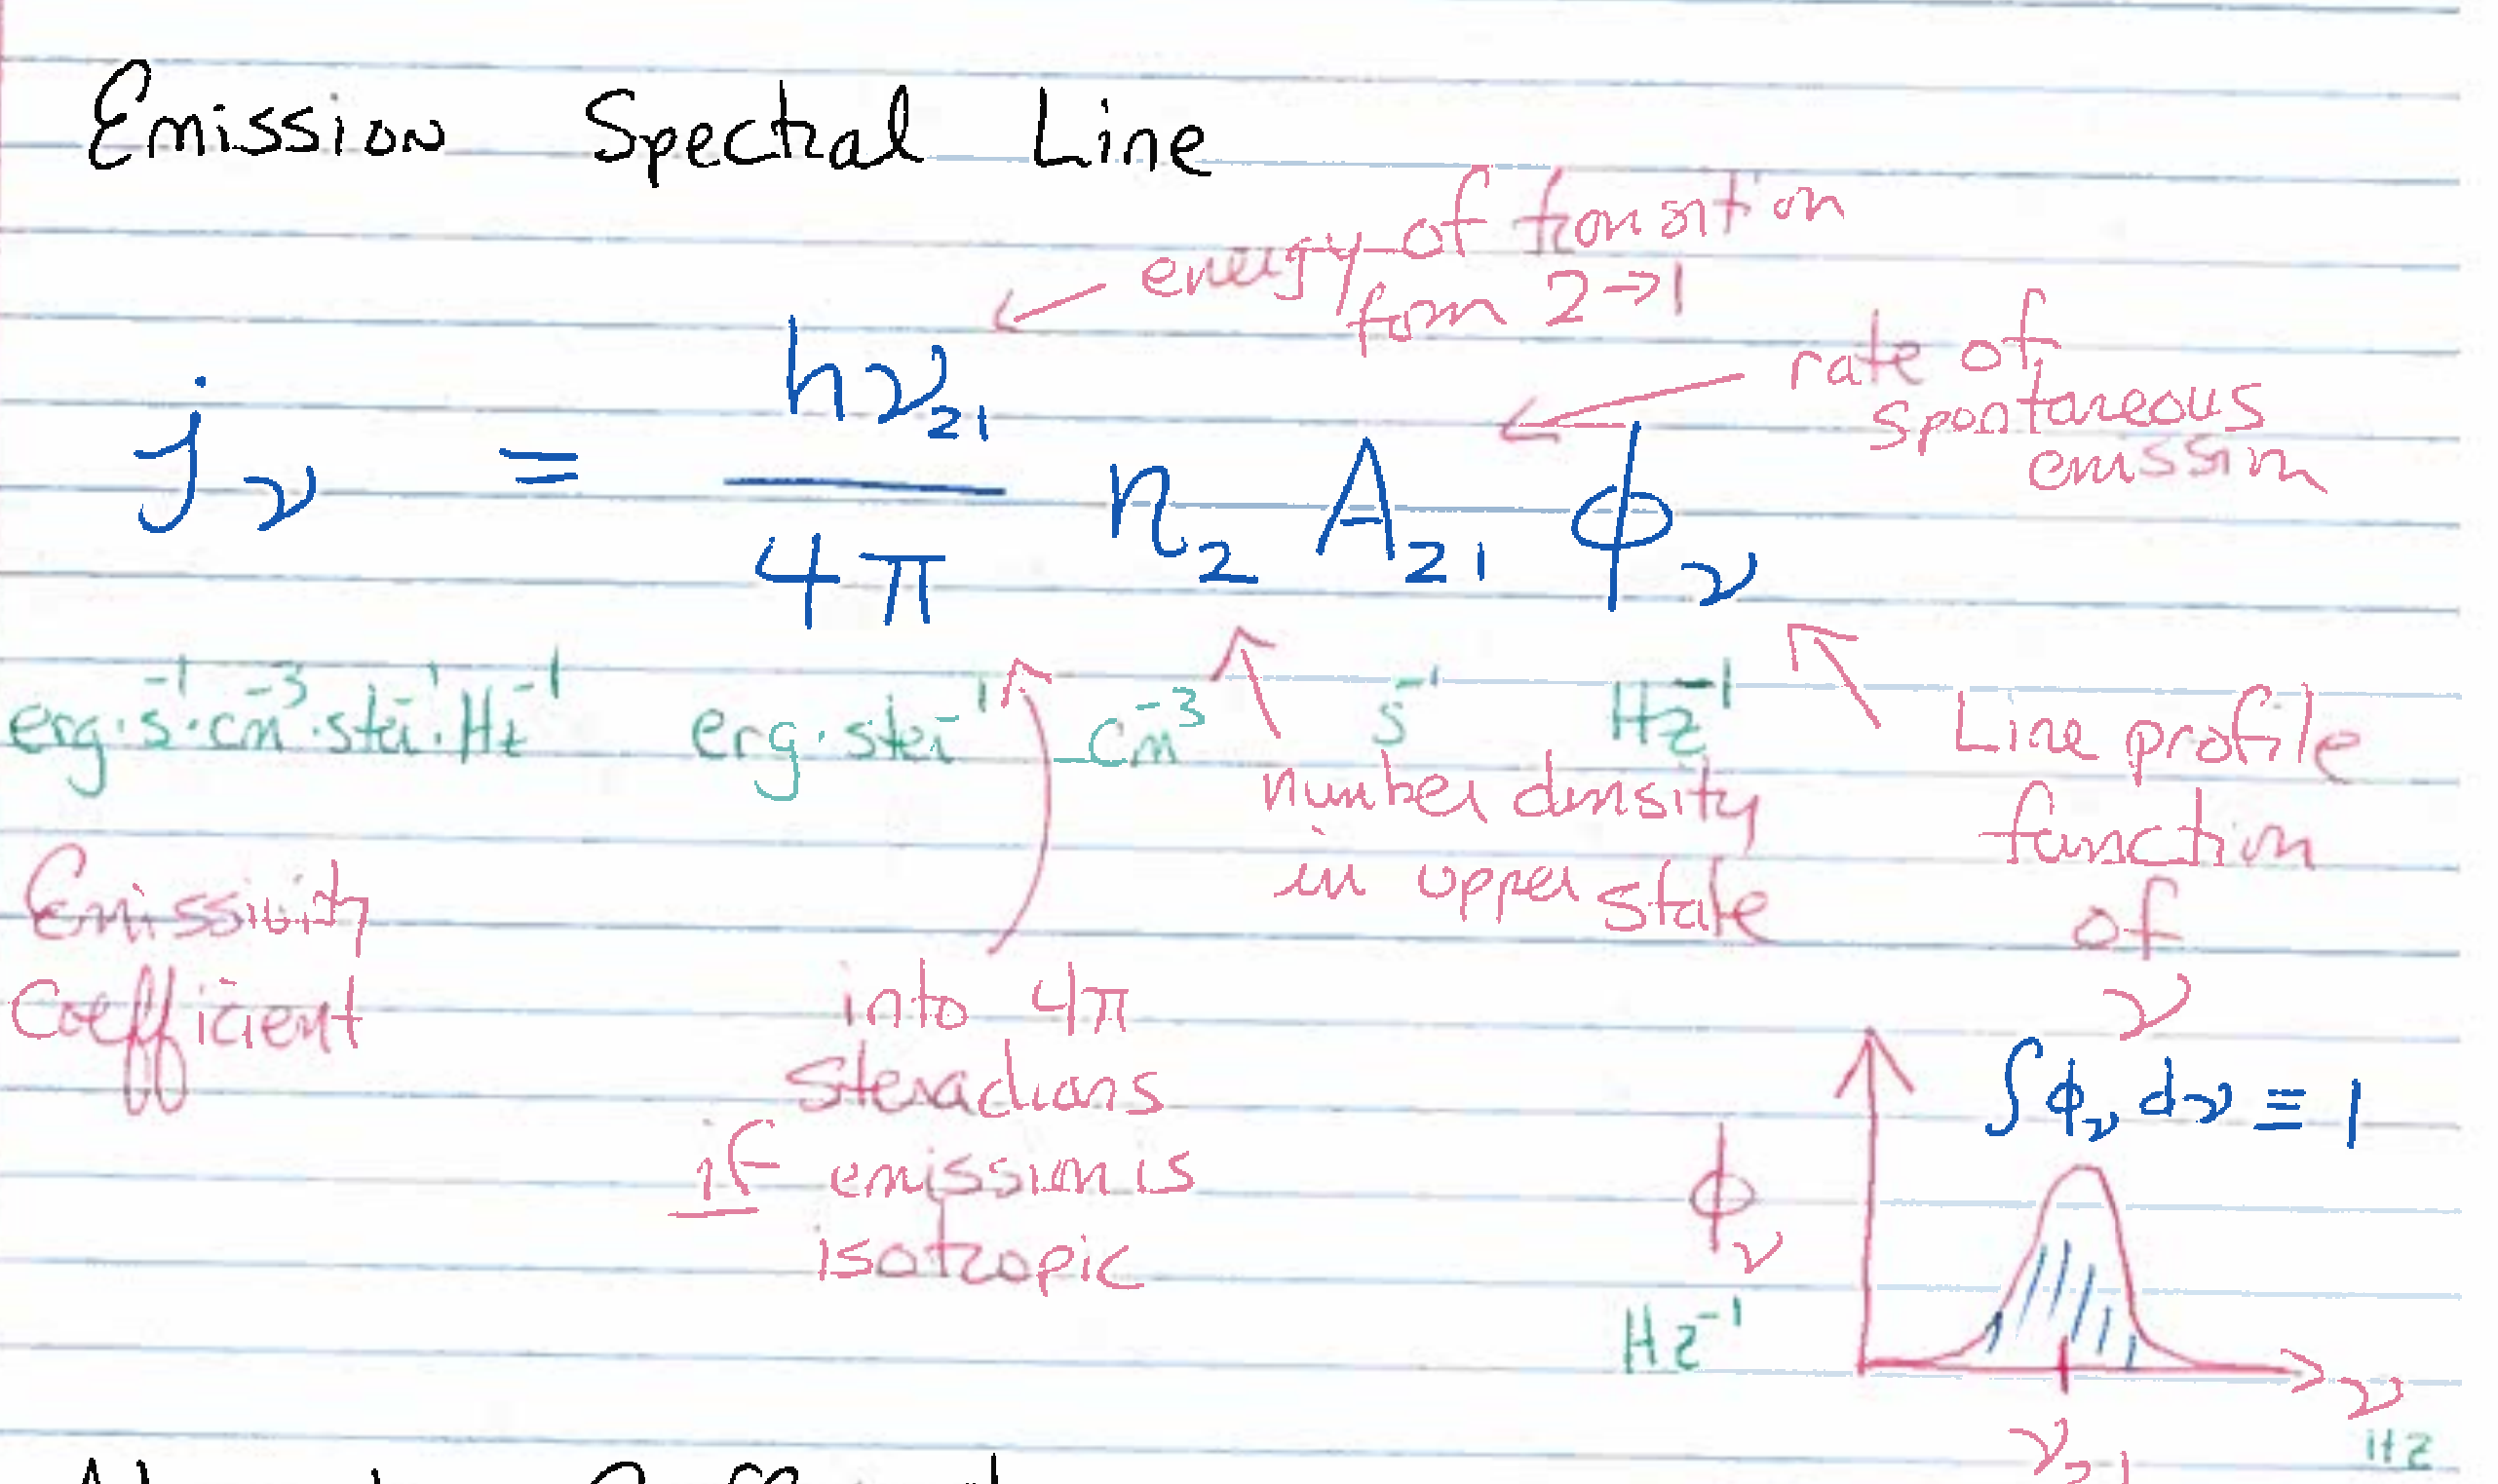
\includegraphics[scale=.5]{emission.png}

\subsection{Spontaneous Emission}

Spontaneous emission is the processes in which a atom/molecule transitions from an excited energy state to a lower energy state, emitting a photon. 
\\$\chi_\nu \longrightarrow h\nu + \chi_l$

When studying radiative processes, we usually use the emission coefficient $j_\nu$ to include in the equation the gain in intensity due to this emission. Then we have:

$j_\nu = \frac{dE}{dV d\Omega dt d\nu}$

$j_\nu = \frac{dI_\nu}{dS}$

$[j_\nu] = erg s^{-1} cm^{-2} str^{-1} Hz^{-1}$

\subsection{Stimulated Emission}

Stimulated emission is when an incoming photon interacts with an atomic electron and makes it drop to a lower energy level. The energy that this process releases goes to the electromagnetic field, creating a new photon with all the same properties as the previously incoming photon. Spontaneous emission is different because it does not relate to the electromagnetic field.

$\chi_\nu + h\nu \longrightarrow \chi_l + 2h\nu$

\subsection{Absorption}

Absorption is the processes in which a atom/molecule gets excited by an incoming photon and transitions from a lower energy state to a more energetic one.

$\chi_l + h\nu \longrightarrow \chi$

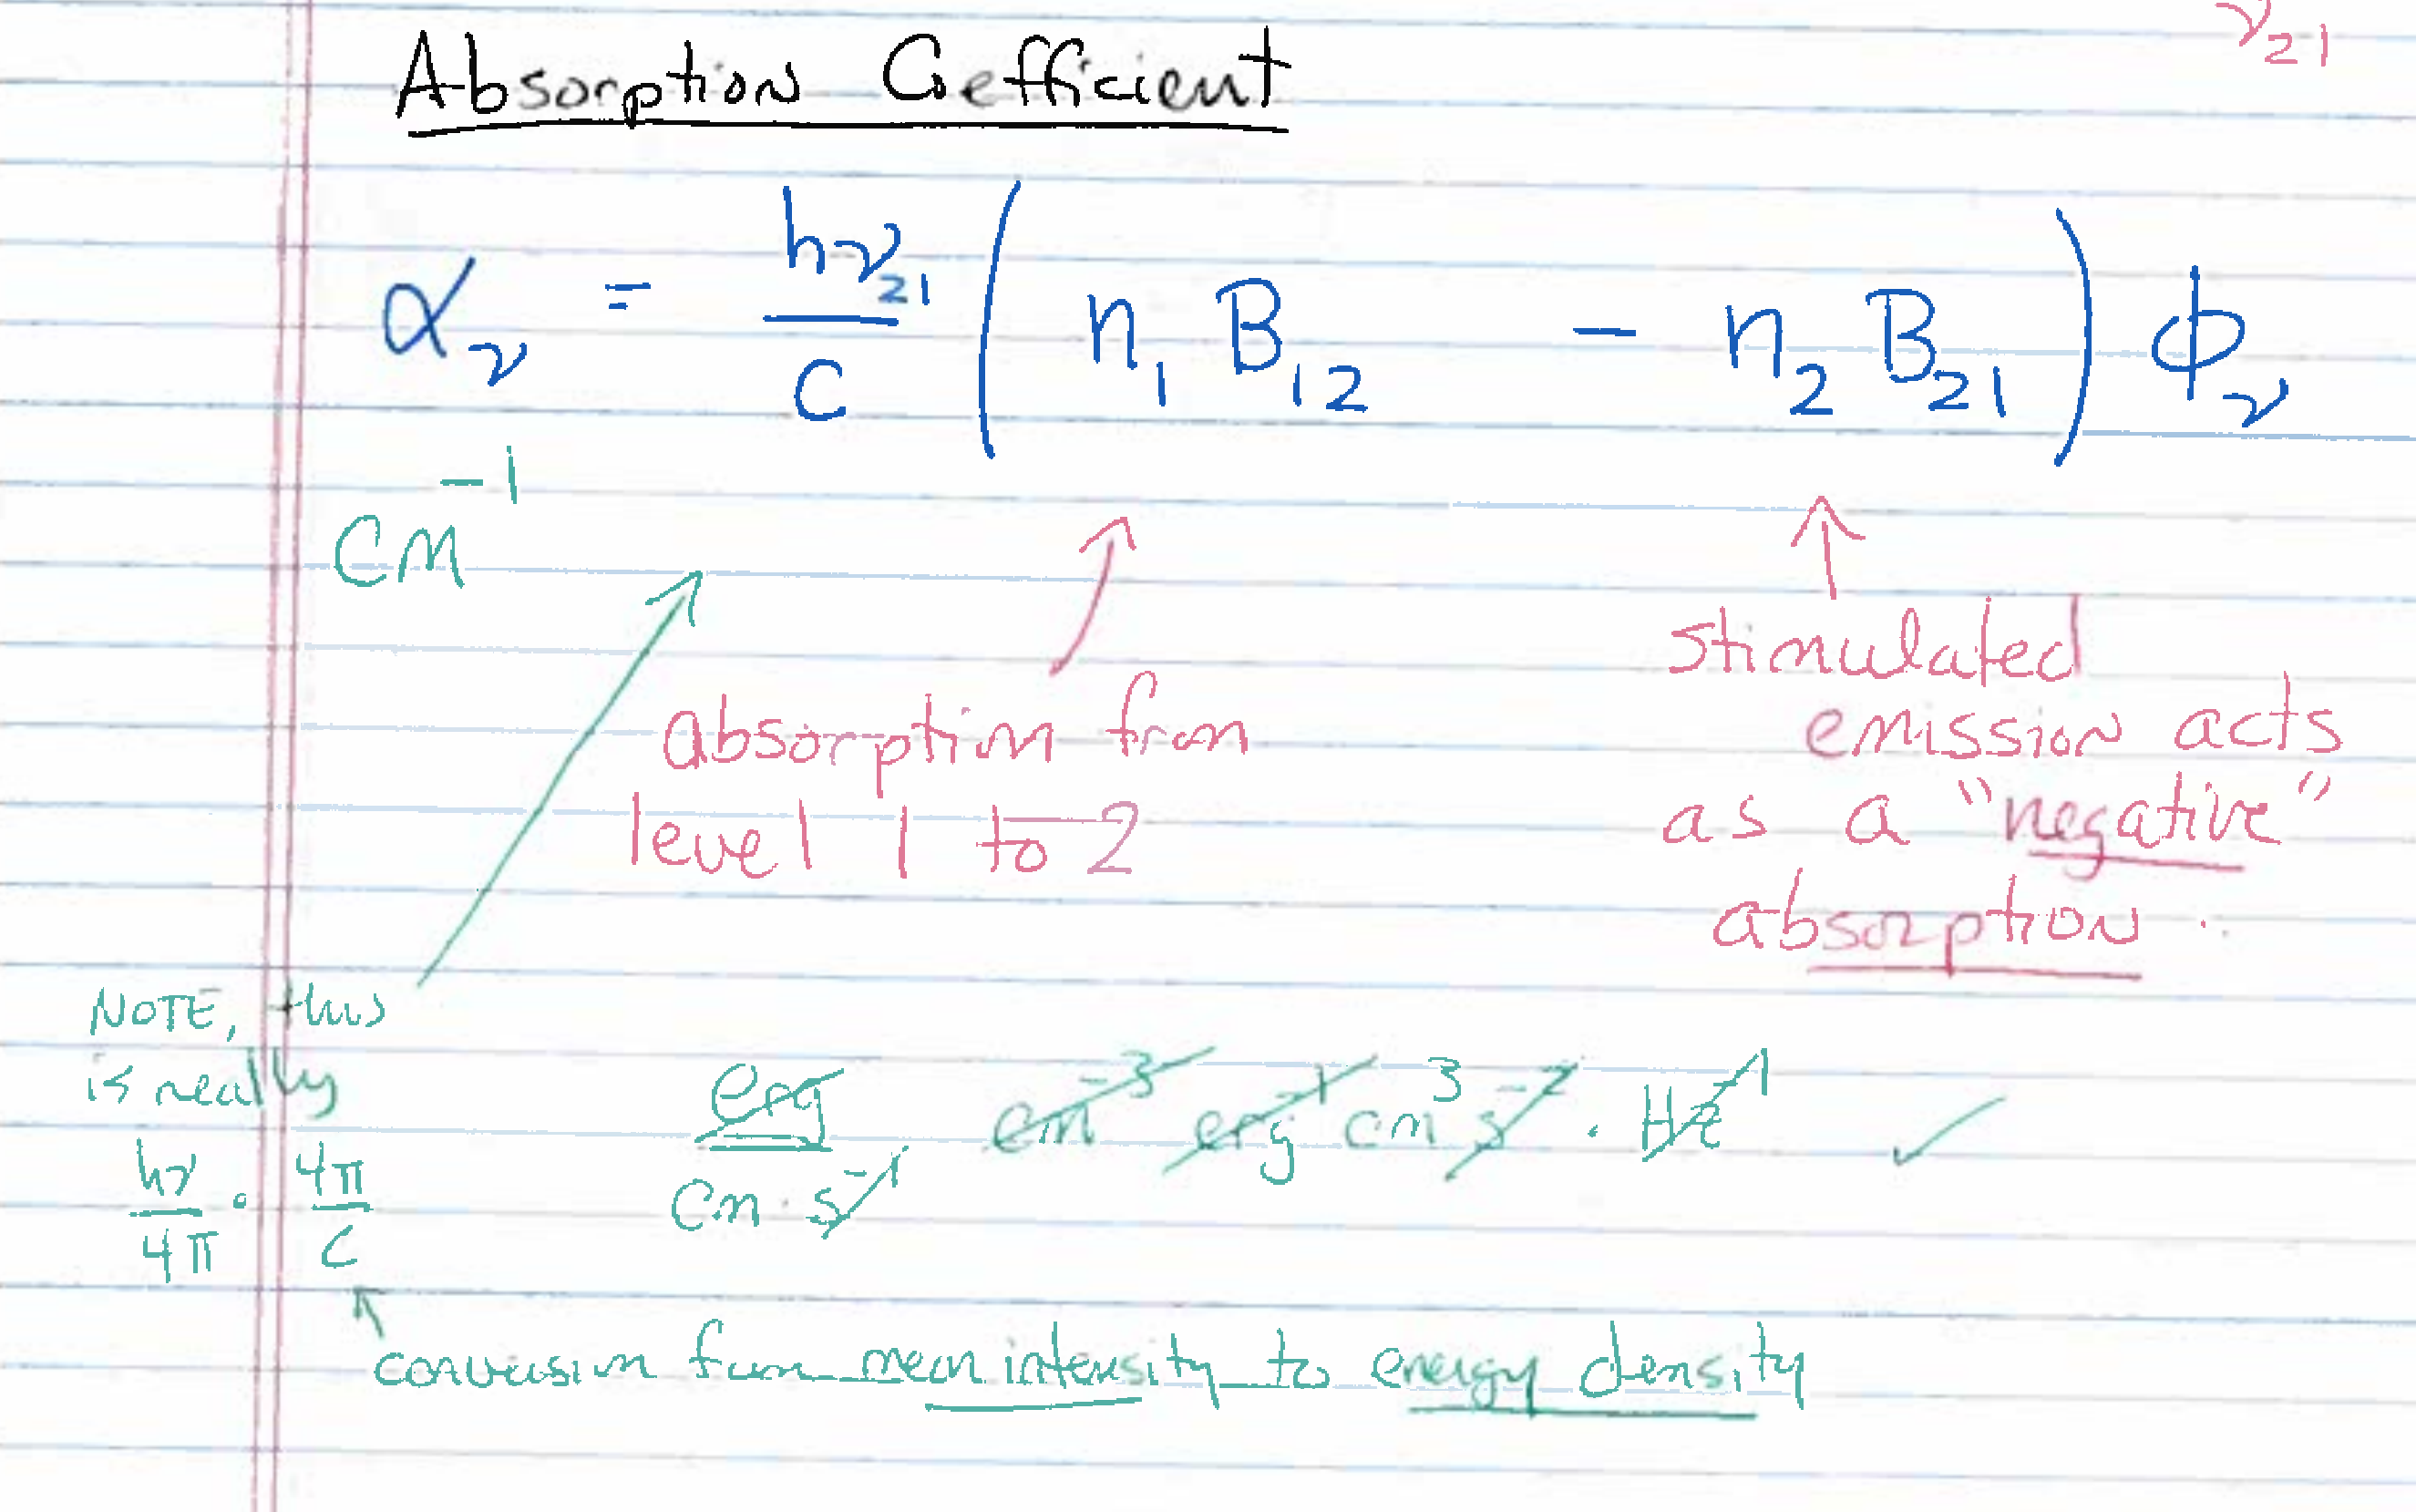
\includegraphics[scale=.5]{absorption.png}

\section{Absorption Cross-Section}
The relation between the monochromatic absorption cross section and a normalized
line profile $\phi_\nu$.
$\sigma_{lu}(\nu) = \frac{g_u}{g_l}\frac{c^2}{8\pi\nu^2_{lu}} A_{ul}\phi_\nu$
with
$\int \phi_\nu dv = 1.$

\section{Line Broadening Mechanisms}

    \subsection{Natrual Line Width}
    
        Lorentz Profile (Cauchy distribution):
        
        $ \phi_{\nu} = \frac{4 \gamma_{\rm UL}}{16 \pi^2 (\nu - \nu_{\rm UL})^2 + \gamma_{\rm UL}^2}$
        
        $\gamma = \sum_{Ej < Eu} A_{\rm uj} + \sum_{Ej > Ei} A_{\rm ij}$
        
        FWHM $ = \frac{\gamma_{\rm UL}}{2 \pi}$
        
        $\Delta v = \frac{c \Delta \nu}{\nu_{\rm UL}} = \frac{\gamma_{\rm UL} \lambda_{\rm UL}}{2 \pi} $
    
    \subsection{Doppler Broadening Profile}
    
        Gaussian Profile:
        
        $P_{\Vec{v}} = \frac{1}{\sqrt{2 \pi}} \frac{1}{\sigma_{\Vec{v}}} 
            e^{-(\Vec{v} - v_{\rm 0})^2 / 2 \sigma^2} $ 
            
        Here $\Vec{v}$ is the velocity and $\sigma$ is the 1D velocity dispersion.
        
    \subsection{Line Profile}\label{sec:line_profile}
    
        The line profile function can be thought of as "A probability function where a photon was emitted and can be absorbed". There are profiles for emitters and absorbers that determine the frequencies at which each emits or absorbs.
    
        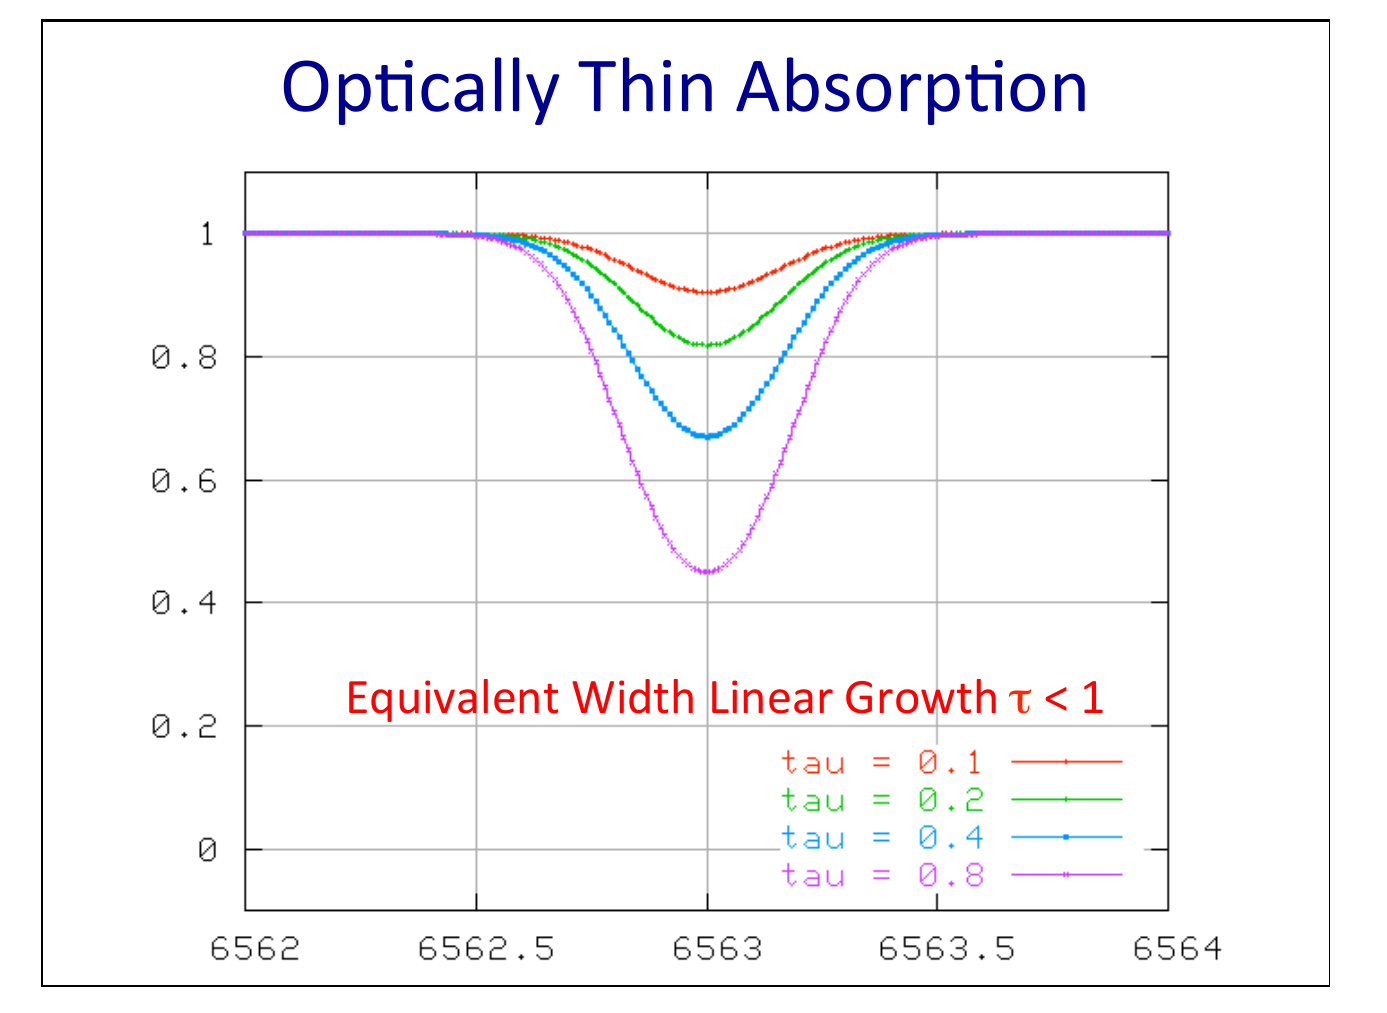
\includegraphics[scale=.5]{thin.png}
        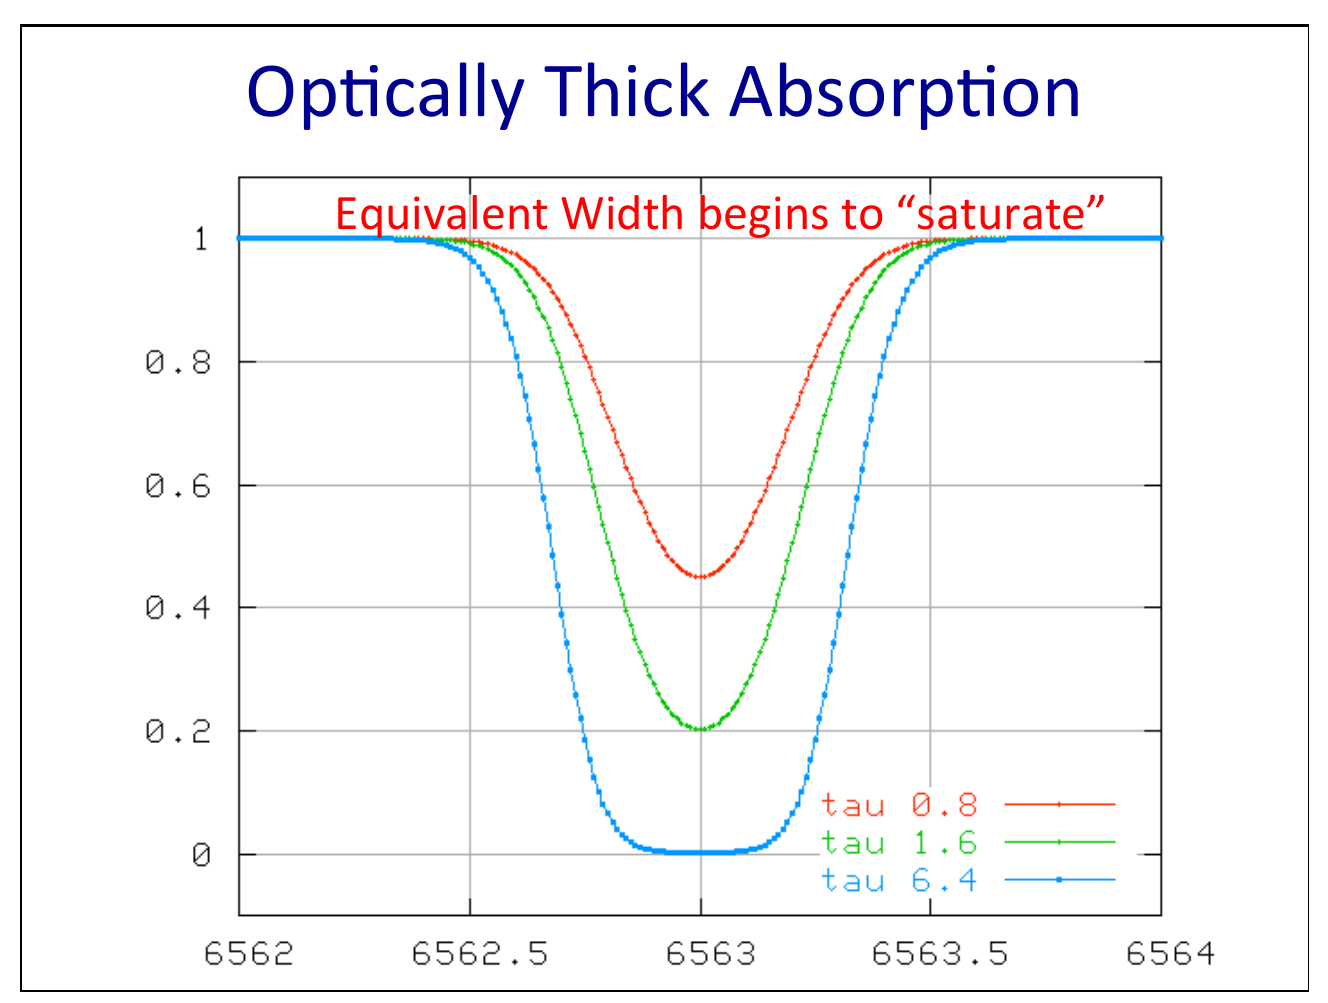
\includegraphics[scale=.5]{thick.png}
        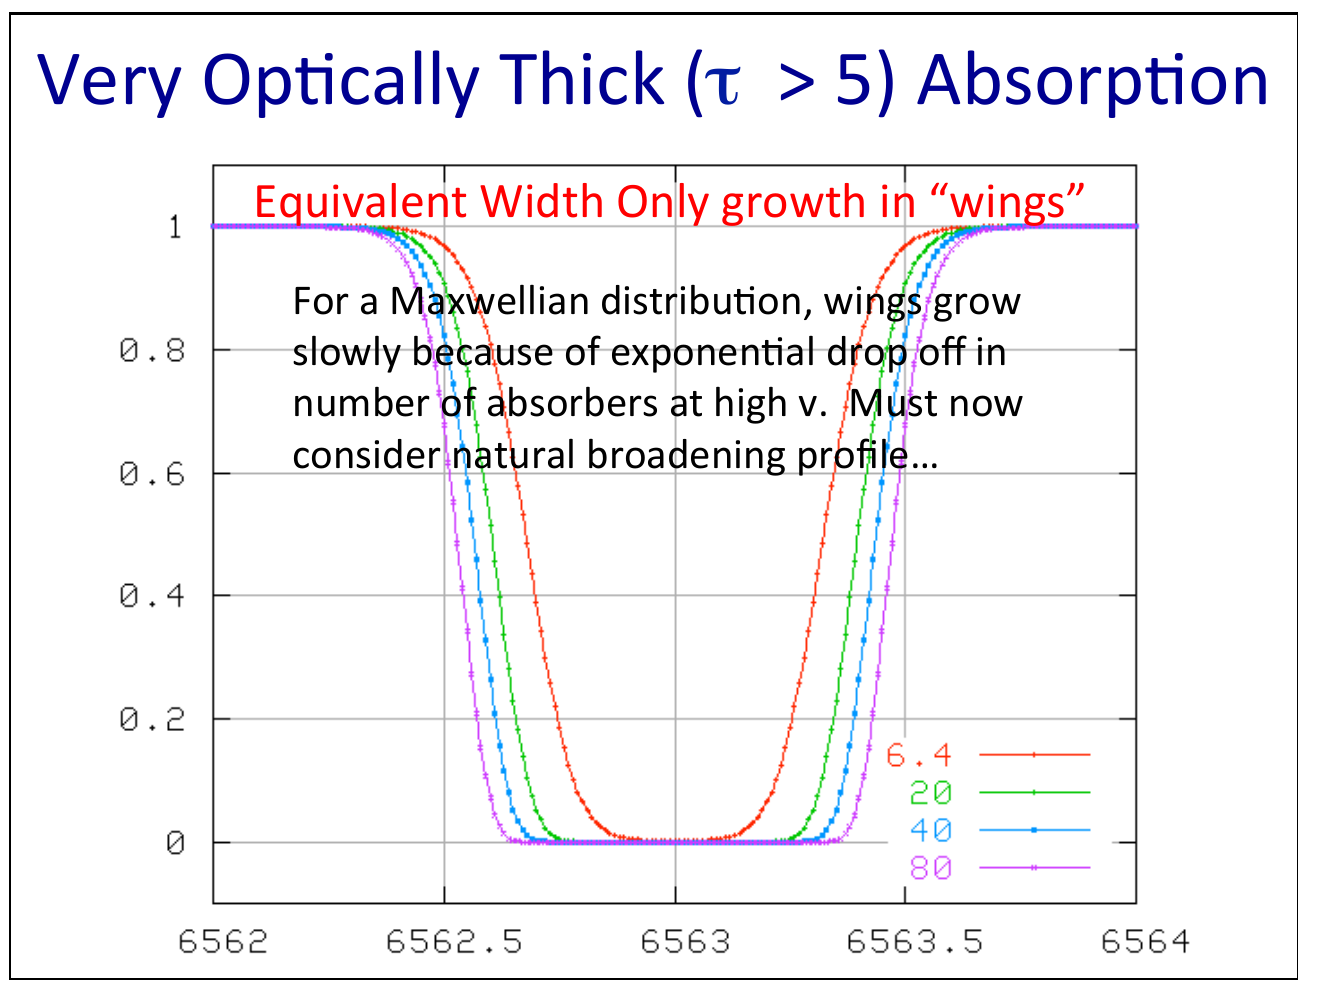
\includegraphics[scale=.5]{very_thick.png}

        The convolved line profile for both kinds of broadening effects:
        
        $ \phi = \int dv \; P_{\Vec{v}}(\Vec{v}) \frac{4 \gamma_{\rm UL}}{16 \pi^2 [\nu - (1-\nu) / (c \nu_{\rm UL}^2) ] + \gamma_{\rm UL}^2}$

\pagebreak

\chapter{Radiative Transfer}
\section{Definitions and Equations}
\begin{figure}
    \centering
    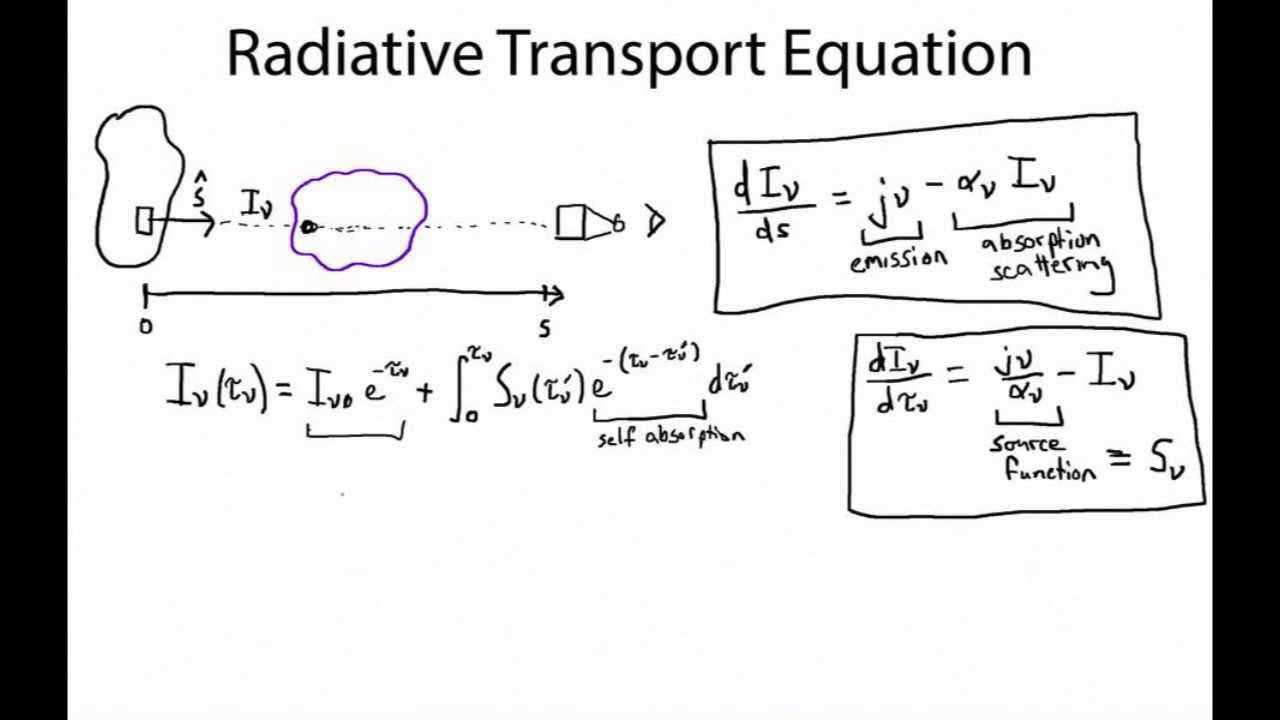
\includegraphics[scale=0.35]{maxresdefault.jpg}
    \caption{Accurate Figure}
    \label{fig:my_label}
\end{figure}
\begin{itemize}
    \item{Intensity: brightness of a ray as it passes through a medium. The units of intensity are [ergs / s / cm$^{2}$ / Hz/ str].
    \begin{align}
    I = \frac{dE}{dA\;d\Omega\;dt\;d\nu}
    \end{align}
    }
    \item{Radiative Transfer: How the intensity from some source interacts with material along the line of sight. This can involve absorption, emission, and scattering.
    \begin{align}
    I_{\nu} = I_{0} e^{-\tau_{\nu}} + S_{\nu} (1 - e^{-\tau_{\nu}})
    \end{align}
    }
    \item{Optical Depth: dimensionless quantity, tells how much the material has absorbed along line of sight.
    \begin{align}
        d\tau_{\nu} = \alpha_{\nu} ds = \kappa_{\nu} \rho ds
    \end{align}
    Where, $\kappa_{\nu}$ and $\rho$ are the opacity and density respectively.
    }
    \item{Source Function: The ratio of the emissivity to absorption coefficient. These are intrinsic to the material. In the limit of local thermodynamic equilibrium, the source function becomes a blackbody.
    \begin{align}
    S_{\nu} = j_{\nu} / \alpha_{\nu} = \frac{n_{u} A_{u \ell}}{n_{\ell} B_{\ell u} - n_{u} B_{u \ell}}
    \end{align}
    }
    \item{Blackbody Function: Intensity at a specific frequency due to the temperature of the material.
    \begin{align}
        B_{\nu} = \frac{2h\nu^{3} / c^{2}}{e^{h\nu/kT} - 1}
    \end{align}
    }
    \item{Thermal emission: occurs when collisional processes dominate over radiative processes. Stats given by Maxwell-Boltzmann statistics so that S$_\nu$ \rightangle B$_\nu$. Becomes blackbody when optically thicc
    \begin{align}
        \frac{n_{u}}{n_{\ell}} = \frac{g_u}{g_\ell}e^{-h\nu/kT}
    \end{align}
    Where $n$ describes the level populations, and $g$ are the degeneracies in each energy level.
    }
    \item{Rayleigh-Jeans Approximation: The Planck function can be approximated using this equation at low frequencies ($h\nu<<kT$).
    \begin{align}
    I_{\nu}^{\rm RJ} = \frac{2\nu^{2}}{c^{2}} kT
    \end{align}
    }
    \item{Wien's Approximation: The Planck function can be approximated using this equation at high frequencies ($h\nu>>kT$).
    \begin{align}
    I_{\nu}^{W} = \frac{2h\nu^{3}}{c^{2}}e^{-h\nu/kT}
    \end{align}
    }
    \item{Specific Energy Density:
    \begin{align}
    U_{\nu} = \frac{I_{\nu}}{c}
    \end{align}
    }
    \item{Angular Averaged Intensity:
    \begin{align}
    J_{\nu} = \frac{1}{4\pi} \int I_{\nu} d\Omega
    \end{align}
    }
\end{itemize}

\section{Kirchoff's Laws}
\begin{itemize}
    \item{
    \begin{enumerate}
        \item{No background emission ($I_{0} = 0$):
        \begin{align}
        I_{\nu} = S_{\nu} (1 - e^{-\tau_{\nu}})
        \end{align}
        \begin{enumerate}
            \item{Optically thin ($\tau << 1$). $S_{\nu}$ goes to $B_{\nu}$ in thermal equilibrium.
            \begin{align}
            I_{\nu} = S_{\nu}\tau_{\nu}
            \end{align}
            }
            \item{Optically thick ($\tau >> 1$). $I_{\nu} = S_{\nu} = B_{\nu}$ in local thermodynamic equilibrium.}
        \end{enumerate}
        }
        \item{Background emission
        \begin{enumerate}
            \item{Optically thin:
            \begin{itemize}
                \item{If $I_{0} > S_{\nu}$, we see an absorption line:
                \begin{align}
                    I_{\nu} = I_{0} - \tau_{\nu} (I_{0} - S_{nu})
                \end{align}
                }
                \item{If $S_{\nu} > I_{0}$, we see an emission line:
                \begin{align}
                    I_{\nu} = I_{0} - \tau_{\nu} (S_{nu} - I_{0})
                \end{align}
                }
            \end{itemize}
            }
            \item{Optically thick:
            \begin{align}
                I_{\nu} = S_{\nu}
            \end{align}
            }
        \end{enumerate}
        }
    \end{enumerate}
    }
\end{itemize}

\section{Scattering}

    \begin{align}
        \frac{dI_{\nu}}{ds} = -(\alpha_{\nu} - \sigma_{\nu,s}) (I_{\nu} - B_{\nu})
    \end{align}
    Where, $\sigma_{\nu,s}$ is the absorption cross-section.
    \begin{align}
        \ell_{*} \simeq \sqrt{N}\ell
    \end{align}
    Where $\ell$ is the mean free path, $N$ is the number of scattering events, and $\ell_{*}$ is the displacement from the center.
    \begin{align}
        \ell = \frac{1}{n\sigma}
    \end{align}
    The number of scattering events can be approximated as
    \begin{align}
        N \sim 1 - e^{-\tau_{\nu}}
    \end{align}


\pagebreak
\chapter{Stellar Atmospheres}

\section{Radiation Pressure}

Further Reading: Draine 41.7 


\begin{equation}
    P_{rad} = \frac{4\pi}{3}I_{\lambda}d_{\lambda}
\end{equation}
\begin{equation}
    P_{rad} = \int \frac{4 \pi}{3} \sigma T^{4}
\end{equation}
Radiation Pressure as a function intensity, and then of time. 


\section{Plane Parallel Atmosphere}

Definition: A \underline{plane parallel} atmosphere is one where the physical properties only change in the z-direction.\newline
Definition: A \underline{grey atmosphere} is one where $\tau$ is not dependent on $\nu$. \newline
Thus, because $S_{\nu}$ is proportional $ds$, we can also say that $S_{\nu}$ is proportional to $d\tau$ (since $d\tau=\kappa\rho ds$)

\begin{equation}
    S_{\nu} \propto d\tau_{\nu}
\end{equation}

\begin{figure}[h]
    \centering
    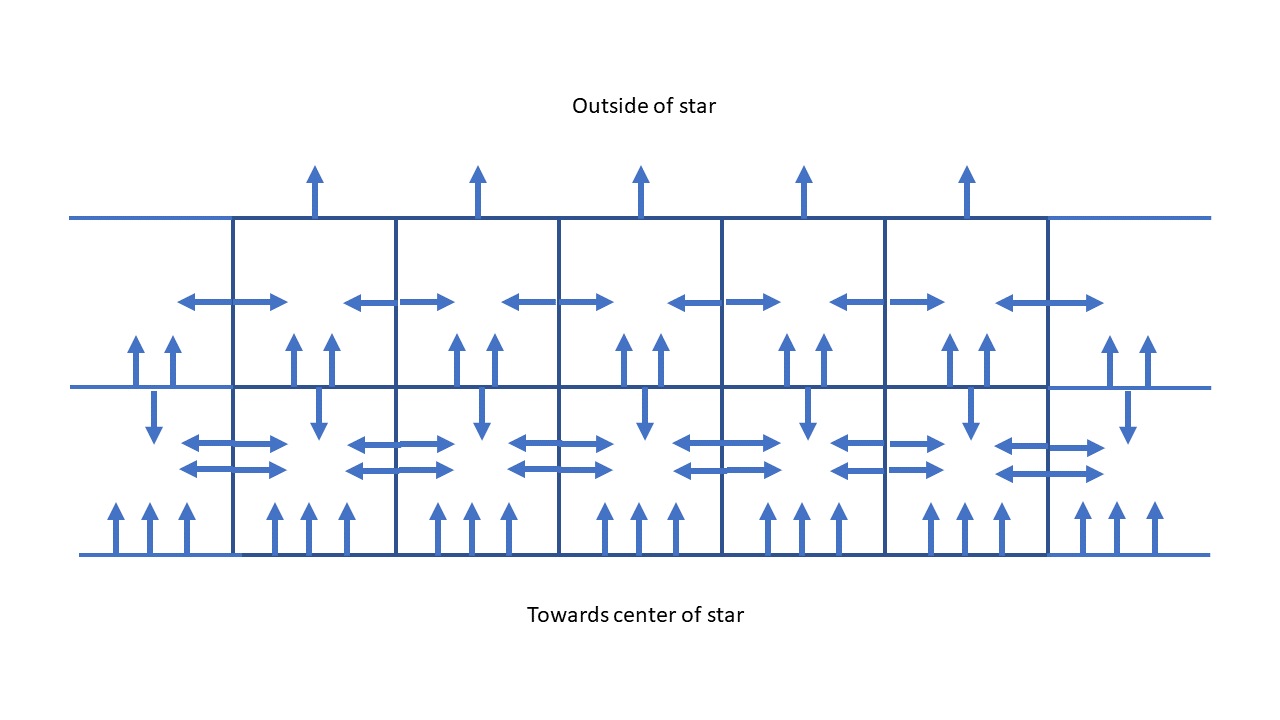
\includegraphics[width=0.7\columnwidth]{radProc_parallel_gmm.png}
    \caption{In order to have emission, there must be more photons etc deeper within the star.}
\end{figure}


\section{Eddington-Barbier Relation}

Approximation: near top of atmosphere ($\tau$<<1),Taylor expand Source function:
\begin{equation}
    S(\tau_{\lambda},v) \approx S_{\lambda}(0) + S_{\lambda}(0) \tau_{\lambda} = a + b \tau_{\lambda}

\end{equation}
Substitute into:

\begin{equation}
    I = \int_{0}^{\infty} S_v T_v e^{-T_v/\mu} d\tau / \mu
\end{equation}

\begin{equation}
    I_{\labmda}(\tau_{\lambda} = 0, \mu > 0) = a + b\mu
\end{equation}

\begin{equation}
    I_{\labmda}(\tau_{\lambda} = 0, \mu > 0) = S_{\lambda}(\tau_{\lambda}= \mu)
\end{equation}

\begin{equation}
    \tau_{\lambda} = \tau_{\lambda} sec \theta = \tau_{\lambda}\mu 
\end{equation}


So intensity I$_{\labmda}$ tells us S$_v$ as a function of $\mu$
\begin{equation}
    I_{\lambda}(τ_{\lambda} = 0, \mu > 0) = S_{\lambda}(τ_{\lambda} = 1)
\end{equation}





\section{Limb Darkening}
Start with the equation of radiative transfer:
\begin{equation}
    \frac{d I_{\nu}}{d \tau_{\nu}}=-I_{\nu} + S_{\nu}
\end{equation}
Multiplying both sides with $e^{-\tau_{\nu}}$ and get:
\begin{equation}
   e^{-\tau_{\nu}} \cdot \frac{d I_{\nu}}{d \tau_{\nu}}=(-I_{\nu} + S_{\nu}) \cdot e^{-\tau_{\nu}}
\end{equation}
Integrate by parts:
\begin{equation}
   \frac{d}{d\tau_{\nu} } (I_{\nu} \cdot e^{-\tau_{\nu}})= -S_{\nu} \cdot  e^{-\tau_{\nu}}
\end{equation}
Integrate w.r.t $\tau_{\nu}$ and get:
\begin{equation}
   I_{\nu}=I_{\nu}(0)e^{-\tau_{\nu}}+\int_{0}^{\tau_{\nu}} S_{\nu} e^{-(\tau_{\nu}\prime-\tau_{\nu})} d\tau_{\nu}\prime
\end{equation}
Assuming that we are all the way into the core, i.e. $\tau_{\nu} \rightarrow \infty$, only the second term would contribute:
\begin{equation}
   I_{\nu}=\int_{0}^{\tau_{\nu}} S_{\nu} e^{-(\tau_{\nu}\prime-\tau_{\nu})} d\tau_{\nu}\prime
\end{equation}
Assuming plane parallel atmosphere:
\begin{equation}
\tau_{\nu}\prime-\tau_{\nu} = \tau_{\nu} \cdot \sec(\theta)
\end{equation}
Plug this in and use the fact that the source function is a linear function of $\tau_{\nu}$ because of isotropic nature of the radiation:
\begin{equation}
   I_{\nu}=\int_{0}^{\infty} (a+b\cdot\tau_{\nu} ) e^{-\tau_{\nu} \cdot \sec(\theta)} \sec(\theta) d\tau_{\nu}
\end{equation}
Evaluate the above integral and get:
\begin{equation}
   I_{\nu}=a_{\nu} + b_{\nu} \cdot \cos(\theta)
   \label{eq:1}
\end{equation}

For the case of the Sun, we have derived the formula for the source funtion:
\begin{equation}
   S_{\nu}=\langle I_{\nu} \rangle =\frac{3 \sigma}{4 \pi} T_{e}^{4} \cdot (\tau_{\nu}+\frac{2}{3}) = a + b\cdot \tau_{\nu}
\end{equation}
Comparing the coefficients, we get the value for $a_{\nu}$ and $b_{\nu}$:
\begin{equation}
   a_{\nu}=\frac{\sigma}{2\pi}\cdot T_{e}^{4}
\end{equation}
\begin{equation}
   b_{\nu}=\frac{\sigma}{4\pi}\cdot T_{e}^{4}
\end{equation}
Put there values into \eqref{eq:1} and we can find the ratio of the specific intensity at angle $\theta$ and angle zero is:
\begin{equation}
   \frac{I_{\nu}(\theta)}{I_{\nu}(0)}=\frac{a_{\nu}+b_{\nu}\cos(\theta)}{a_{\nu}+b_{\nu}}=\frac{2}{5}+\frac{3}{5}\cdot \cos(\theta)
\end{equation}



\section{Curve of Growth}\label{sec:growthcurve}

\fbox{\parbox{\textwidth}{TL;DR How do the equivalent width of absorption lines evolve with increasing number of absorbers $N$?
\begin{itemize}
    \item Weak lines: Doppler broadening, $EW\propto N$
    \item Saturated lines: Doppler broadening, but only in the wings, $EW \propto \sqrt{ln(N)}$
    \item Strong lines: Lorentzian profile begins to dominate due to collisional broadening, $EW \propto \sqrt{N}$
\end{itemize}}}
\begin{figure}
    \centering
    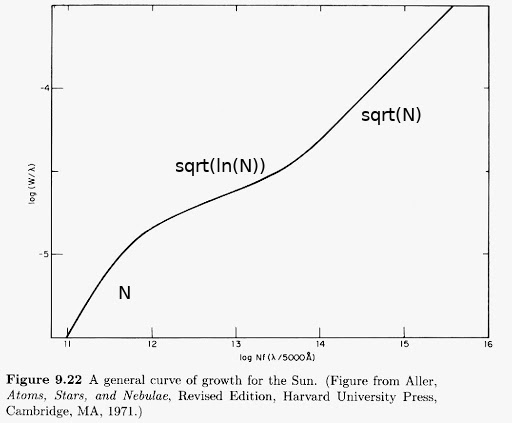
\includegraphics[scale=0.6]{growthcurve.jpg}
    \caption{A labeled, graphical representation of the curve of growth for equivalent widths of absorption lines in the Sun.}
    \label{fig:growth_curve}
\end{figure}

\textbf{More detail:}\newline
Consider an absorption line surrounded by continuum emission at intensity $I_{0}$ and a (reduced) minimum intensity of $I_{\nu}$. Its equivalent width, a measure of the total amount of radiation absorbed in a particular line, is given by the integral of the absorption depth $D$:
\begin{equation}
    EW = \sum_{\nu}D d\nu = D_{\rm max}\sum_{\nu}(1-I/I_{0})d\nu=\sum_{\nu}(1-e^{-\tau})d\nu
\end{equation}
where $\tau$ is the optical depth of the absorber and $D_{\rm  max}$ is the maximum depth of the line. A fundamental question here is, then: How does the equivalent width of an absorption line change as more atoms contribute to it (i.e. the number of absorbers $N$ increases), and what forms can these contributions take?\newline
For a small amount of absorbing atoms (i.e. low density, weak lines), the dominant physical process governing line width is Doppler broadening. Taking the low density of the absorber to mean $\tau \ll 1$, the absorption depth $(1-e^{-\tau})$ is approximately $\tau$. The optical depth itself follows a Voigt profile (see \ref{sec:line_profile}), with a Gaussian center due to random motions causing red/blueshift but Lorentzian wings due to collisions; however, since Doppler broadening dominates in this low-optical-depth regime, we can assume it instead follows a completely Gaussian profile around the central line frequency. When integrated to give the EW, this gives \framebox{$EW \propto N$}. (Maybe a quicker way to conceive of this is as follows: since $\tau=\kappa\rho s$ for some assumptions about the cloud, the optical depth varies linearly with density, and the equivalent width varies linearly with the optical depth while it is low.)\newline
However, increasing the number of absorbers will eventually end in the complete absorption of the initial intensity. At this point ($\tau\approx 5$), the EW cannot increase by decreasing intensity at the exact frequency of the line, so it must come from the wings of the Gaussian instead, as the optical depth is still not high enough for collisional processes (and therefore, the Lorentzian wings) to significantly matter (although they will in a little bit.) What increases there are in the EW, then, are much slower: to a good approximation, \framebox{$EW \propto \sqrt{ln(N)}$}.\newline
As the density continues to rise, collisions will become increasingly important; the resulting distribution of velocities will lead to an optical depth that falls off as $(\nu-\nu_{0})^{-2}$ for $\nu$ sufficiently far away from the line frequency $\nu_{0}$, which at this point are the only unsaturated regions. This shape is clearly not a Gaussian, so it follows that the EW will evolve differently: substituting the Lorentzian profile into the EW integral will yield \framebox{$EW \propto \sqrt{N}$}.

\pagebreak
\chapter{Statistical Equilibrium: Bound-Bound Transitions}
\input{statistical_equilibrium.tex}
\pagebreak
\chapter{Statistical Equilibrium: Bound-Free Transitions (i.e. Photoionization)}
\input{photoionization.tex}
%\chapter{Electricity and Magnetism}
%R\&L Chapter 2
\pagebreak
\chapter{Free-Free Emission}
\input{freefree.tex}
\pagebreak
\chapter{Synchrotron Radiation}
\input{synchrotron.tex}


\end{document}
 
